\chapter{PROBLEMA}
Diante do exposto, pretendemos realizar uma análise a respeito do uso de Redes Neurais Artificiais abordando o aprendizado não supervisionado para a detecção de intrusões em ambientes IoT domésticos, também responder a seguinte pergunta: Em relação ao desempenho e usabilidade, o uso de Redes Neurais Artificiais para proteção de redes domésticas é uma escolha viável?

\chapter{HIPÓTESES}
Com um software inteligente baseado em Redes Neurais, é possível reconhecer os padrões e comportamentos de uma rede doméstica, e diferenciar um trafego normal de um ataque.

\chapter{OBJETIVO GERAL}
Avaliar a eficiência da implementação de um Sistema de Detecção de Intrusão baseado em Redes Neurais Artificial não supervisionadas, em hardwares domésticos.

\section{OBJETIVOS ESPECÍFICOS}
\begin{itemize}
    \item Realizar a implementação do Sistema de Detecção de Intrusão para redes domésticas baseado no IDS Kitsune;
    \item Verificar o desempenho do IDS em hardwares comuns em residencias;
    \item Analisar a eficiência do IDS com ataques simulados em ambientes IoT Domésticos;
    \item Realizar uma investigação sobre a taxa de erro do algorítimo em ambientes IoT domésticos;
    \item Apresentar os resultados do Sistema de Detecção de Intrusão, para assim, validar a eficiência e precisão do algoritmo em ambientes domésticos; 
 \end{itemize}

\chapter{JUSTIFICATIVA}
Ao observarmos a complexividade da prevenção e detecção de ataques, visualizamos o problema da rápida e constante mudança da maneira que esses ataques acontecem. Por isso é essencial que os métodos de segurança sejam constantemente atualizados. Uma ferramenta útil são os Sistemas de Detecção de Intrusão (IDS), que são softwares que monitoram o tráfego, e tomam ações caso exista um comportamento incomum na rede.

Com a flexibilidade dos IDSs, é possível trabalhar em conjunto com outros sistemas, como Firewalls ou hardwares, ou integra-los a Redes Neurais Artificiais (RNA), possibilitado que eles tenham uma tomada de decisão e aprendizado.
Redes Neurais Artificiais não supervisionadas, são um ponto chave em IDSs, pois não se faz necessário o tempo e esforço para atualizar manualmente o Sistema de Detecção de Intrusão, já que o mesmo aprende de forma incremental a partir dos dados e padrões. 

Para que um IDS seja implementado em um ambiente domestico, é importante que ele exija pouco uso de processamento, pois na maioria dos casos, os hardwares domésticos são menos robustos e possuem um sistema simples. O algorítimo Kitsume, usa uma complexividade baixa em sua execução, trazendo um menor uso de processamento \cite{kitsune}.

Kitsune é um IDS baseado em Redes Neurais, que utilizaremos como base de pesquisa, pois além de ser um Software de código aberto, possui uma robusta abordagem de aprendizado não supervisionado, usando de Autoencoders para diminuir a complexidade dos processos.

Com esta pesquisa, espera-se contribuir com um relatório sobre a eficácia do método de aprendizado de máquina não supervisionado para soluções de segurança de redes domesticas, e apresentar um estudo aprofundado sobre o impacto de ataques de intrusão.

\chapter{REFERENCIAL TEÓRICO}
\section{Internet das Coisas (IoT)}
O termo Internet das Coisas se refere a conexão de vários objetos por meio da internet. Dispositivos IoT são capazes de interagir de maneira autônoma, possuindo uma capacidade “inteligente” de receber e processar informações pela rede. Em ambientes domésticos, estes dispositivos são responsáveis por automatizar tarefas do dia a dia \cite{gokhale2018introduction}.
 
\subsection{Segurança em IoT}
Com a vasta possibilidade de conexão em todo ambiente, aumentam também as vulnerabilidades a ataques. Dispositivos IoT muitas vezes não são projetados para terem um sistema robusto de segurança, pois o envio de informações precisa ser rápido, assim deixando as questões de segurança em segundo plano ou inexistentes. Nessas condições, estes dispositivos acabam sendo uma porta de entrada para ataques \cite{Anthi}. 

\hfill
\newcolumntype{L}{>{\RaggedRight\arraybackslash}X}
\begin{table}[!hbt]
\renewcommand\thetable{1}
\setlength\tabcolsep{3pt} 
\caption{Ataques comuns em redes IoT}
\centering
 \begin{tabularx}{\textwidth}{@{}*{4}{L} @{}} 
 \toprule
 Ataque & Alvo & Consequência & Técnica \\ [0.5ex]
 \midrule
 Negação de Serviço &
 Dispositivos IoT conectados a rede &
 Torna os dispositivos inacessíveis &
 Envia várias requests que nunca são completadas \\ 
 \addlinespace
 Wormholes &
 Localização dos pacotes de rede &
 Cria problemas de privacidades e nas rotas dos pacotes &
 Reencaminha os pacotes copiados dentro da rede \\ 
 \addlinespace
 Ataque de Repetição &
 Informações trocadas na rede &
 Gera altas latências na rede e autenticações falsas &
 Intercepta credenciais e as reenvia para se autenticar falsamente \\ 
 \addlinespace
 Ataque Sybil &
 Integridade de dados e recursos &
 Gera altas latências na rede &
 Cria credenciais faltas e opera como um usuário normal \\ 
 \addlinespace
 \bottomrule
\end{tabularx}
\fonte{\citeonline{Pavlovic}} 
\end{table}

\section{Protocolos de Rede}
Atuamente, a conexão de dispositivos IoT são principalmente baseadas no protocolo TCP/IP, sua premissa é conectar dispositivos na rede independente de sua arquitetura e recursos. \cite{Djama}

\subsection{Protocolo de Internet (IP)}
O protocolo IP é responsável pelo roteamento/encaminhamento de pacotes, este também é chamado de protocolo sem conexão, pois não garante a entrega dos pacotes ao destinatário. \cite{alqahtani2013tcp}

\subsection{Protocolo de Controle de Transmissão (TCP)}
O protocolo TCP trabalha juntamente ao IP, pois é responsável por dividir os dados em seguimentos antes que estes passem pelo IP, que os reagrupa e encaminha. TCP é considerado mais confiável pois garante a entrega dos pacotes aguardando uma resposta do destinatário para confirmar o recebimento. \cite{alqahtani2013tcp}

\section{Conteúdo de Pacotes TCP/IP}
Os pacotes possuem cinco campos principais em seu cabeçalho: IP de origem, IP de destino, porta de origem, porta de destino e protocolo. Estes campos são responsáveis por identificar a quem pertencem estes pacotes \cite{sbrc_estendido}.

\begin{figure}[h]
\renewcommand\thefigure{1}
\centering
\caption{Modelo de Pacote}
\frame{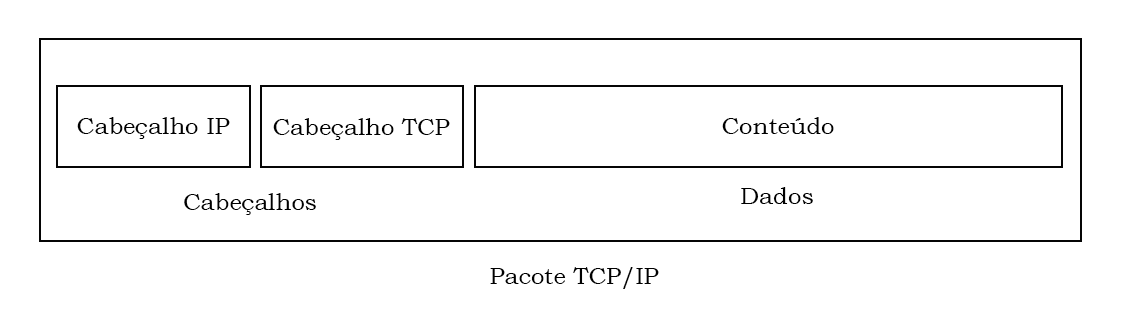
\includegraphics[scale=0.37]{imagens/dados.png}}
\label{fig:exemplo}
\fonte{\citeonline{Jasim}, Adaptado} 
\end{figure}

O conteúdo dentro dos cabeçalhos é essencial para a identificação de ataques, pois possuem informações importantes que podem ser analisadas por IDSs.

\section{Sistema de detecção de intrusão}
Sistema de Detecção de Intrusão (IDS) é um software ou hardware que analisa o trafego de rede buscando comportamentos maliciosos ou violação de regras. Ele funciona analisando os pacotes de rede ou o comportamento dos mesmo para assim identificar anomalias. \cite{CHORAS2021705}

Outra abordagem são os IDSs baseados em Redes Neurais Artificiais (RNA), estes são mais complexos e tem a habilidade de aprender a partir de exemplos, generalização ou dados incompletos \cite{Anitha}. Assim estes podem identificar e aprender quais ações são normais ou maliciosas.

\section{Rede Neural Artificial}
As redes neurais artificiais são técnicas computacionais que usam regras matemáticas incrementais para adquirir conhecimento através de experiencias. Por isso possibilitam trabalhar com modelagem e resolução de
problemas com dados não organizados, treinando, testando e validando um conjunto de dados na entrada visando um objetivo de saída \cite{barros2018avaliaccao},

Para a implementação de um IDS baseado em Redes Neurais Artificiais, é preciso de um modelo de treinamento que ajudará a classificar os pacotes do tráfego de rede. Para isso os dados têm um papel fundamental, quanto mais dados são analisados, melhor será o modelo de treinamento, tornando a base de classificação robusta.